% arara: latexmk: { options: [ '-pdf' ] }
% arara: latexmk: { options: ['-c' ] }
\documentclass{article}

\title{Physics C Unit 8 FRQs}
\author{Henry Beveridge}
\date{\today}
\usepackage{amsmath}
\usepackage{tikz}

\begin{document}

\maketitle

\section*{1.}

\subsection*{a.}

\textbf{i.}

\begin{align*}
  E_A &= \int dE_A \\
  &= \int \frac{k dq}{r^2} \\
  &= k \int_0^L \frac{dq}{(a+x)^2} \\
  &= k \int_0^L \frac{\lambda_0 dx}{(a+x)^2} \\
  &= k \lambda_0 \left(\frac{1}{a+x} \Big|_0^L\right) \\
  &= k \lambda_0 \left(\frac{1}{a+L} - \frac{1}{a}\right) \\
\end{align*}

\textbf{ii.}

\begin{align*}
  E_B &= \int dE_B \\
  &= \int \frac{k dq}{r^2} \cdot \frac{a}{r} \\
  &= k \int \frac{a \lambda_0}{(a^2+x^2)^{3/2}} dx \\
  &= k \lambda_0 a \int_{-\frac{L}{2}}^{\frac{L}{2}} \frac{1}{(a^2+x^2)^{3/2}} dx \\
\end{align*}

\textbf{iii.} The magnitude $E_{new}>E_A$ because everything is the same except more charge is concentrated closer
to the point $A$, meaning that the electric field is stronger at point $A$.

\subsection*{b.}
Using a Gaussian surface of a cylinder of radius $a$ and length $l$:

\begin{align*}
  E_B\cdot A &= \frac{Q_{enc}}{\varepsilon_0}\\
  E_B\cdot 2\pi a l &= \frac{\lambda_0 l}{\varepsilon_0} \\
  E_B &= \frac{\lambda_0}{2\pi a \varepsilon_0}
\end{align*}

\newpage
\section*{2.}

\subsection*{a.}

\begin{center}
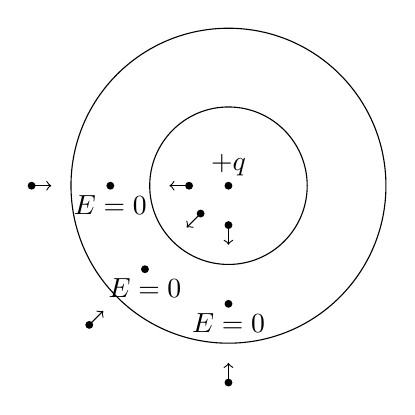
\begin{tikzpicture}
  \draw (0,0) circle (1);
  \draw (0,0) circle (2);

  \fill (0,0) circle (0.05) node[anchor=south] {$+q$};

  \fill (0,-0.5) circle (0.05);
  \fill (0,-1.5) circle (0.05);
  \fill (0,-2.5) circle (0.05);

  \fill (-0.5, 0) circle (0.05);
  \fill (-1.5, 0) circle (0.05);
  \fill (-2.5, 0) circle (0.05);

  \fill (-{0.5/sqrt(2)},-{0.5/sqrt(2)}) circle (0.05);
  \fill (-{1.5/sqrt(2)},-{1.5/sqrt(2)}) circle (0.05);
  \fill (-{2.5/sqrt(2)},-{2.5/sqrt(2)}) circle (0.05);

  \draw[->] (0,-0.5) -- (0,-0.75);
  \draw[->] (-0.5,0) -- (-0.75,0);
  \draw[->] (-{0.5/sqrt(2)},-{0.5/sqrt(2)}) -- (-{0.75/sqrt(2)},-{0.75/sqrt(2)});

  \node[anchor=north] at (0,-1.5) {$E=0$};
  \node[anchor=north] at (-1.5,0) {$E=0$};
  \node[anchor=north] at (-{1.5/sqrt(2)},-{1.5/sqrt(2)}) {$E=0$};

  \draw[->] (0,-2.5) -- (0,-2.25);
  \draw[->] (-2.5, 0) -- (-2.25, 0);
  \draw[->] (-{2.5/sqrt(2)},-{2.5/sqrt(2)}) -- (-{2.25/sqrt(2)},-{2.25/sqrt(2)});
\end{tikzpicture}
\end{center}

\subsection*{b.}

Inside the smaller shell @ $r=\frac{2}{3}R$: $Q_{enc}=q$ and $EA=E_0 \cdot 4\pi\left(\dfrac{2R}{3}\right)^2$

\noindent The inner shell must have charge of $-q$ to result in a field of zero.

\noindent The net charge @ $r=\frac{8}{3}$: $EA=-E_0\cdot 4\pi\left(\dfrac{8R}{3}\right)^2$

\noindent Thus, the outer shell must have a charge of $-16q$ to result in a field of -$E_0$.

\subsection*{c.}

\begin{center}
\begin{tikzpicture}
  \draw[->] (0,0) -- (0,4);
  \draw[->] (0,0) -- (6,0);
  \draw[dashed] (0,2) -- (6,2);

  \node[anchor=north] at (1.5,0) {$R$};
  \node[anchor=north] at (3,0) {$2R$};
  \node[anchor=north] at (4.5,0) {$3R$};

  \fill (1,2.5) circle (0.05);
  \fill (2.5,2) circle (0.05);
  \fill (4,1.5) circle (0.05);

  \draw[domain=0:1.5] plot (\x,{0.5/(\x+0.49999)^2+2.28});

  \draw[domain=1.5:3] plot (\x,2);

  \draw[domain=3:6,range=0:5] plot (\x,{-0.75/(\x-2)^2+1.70});

\end{tikzpicture}
\end{center}

\subsection*{d.}
The only part that would change would be $r>2R$, and there would be no electric field at this point because the enclosed charge would be zero.

\section*{4.}

\subsection*{a.} 

Electric field from Sphere 2 is only in the $-y$ direction, and electric field from Sphere 1 is both in $-x$ and $-y$ directions, with a larger $-y$ 
direction. This means that net electric field is mostly in the $-y$ direction, with a slight skew towards the $-x$ direction.

\subsection*{b.}

$F_q$ is only in the -y direction, so we can use the $-y$ component of the electric field to find the force on the charge.

\begin{align*}
  F_q &= 2 \cdot k \frac{Qq}{r^2} \cdot \frac{y}{r} \\
  &= 2 \cdot k \frac{Qq}{\frac{D^2}{4}+y^2} \cdot \frac{y}{\sqrt{\frac{D^2}{4}+y^2}} \\
  &=  \frac{2kQqy}{\left(\frac{D^2}{4}+y^2\right)^{3/2}} \\
\end{align*}

\subsection*{c.}

This time $F_y$ would be zero because the two fields cancel out, and $F_x$ would be double the force from one sphere. Overall, the magnitude would be 
multiplied by $\dfrac{D}{2y}$




\end{document}
